\RequirePackage{luatex85}
\documentclass{article}
\usepackage{pgfplots}
\usepgfplotslibrary{groupplots}
\pgfplotsset{
 % define the colormap
 colormap={parula}{
   rgb=(0.208100000000000,0.166300000000000,0.529200000000000)
   rgb=(0.969700000000000,0.848138095238095,0.147452380952381)
   rgb=(0.976300000000000,0.983100000000000,0.0538000000000000)
  },
}
\begin{document}
\begin{tikzpicture}
 \begin{groupplot}[
   group style={
     group name=G,
     group size=3 by 1,
     y descriptions at=edge left,
     horizontal sep=20pt % adjust as needed
    },
   enlargelimits=false,
   % !!! I don't know what the part `width("300")' is doing exactly !!!
   width=0.28\textwidth-width("300"),
   height=0.25\textheight,
   scale only axis,
   axis on top,
   grid=both,
  ]
  % add the colorbar to the first groupplot
  \nextgroupplot [
    % it should be horizontal ...
    colorbar horizontal,
    % ... and sampled
    colorbar sampled,
    % define the style of the colorbar
    colorbar style={
      % it should be positioned at ...
      at=(G c1r1.below south west),
      % ... with the anchor ...
      anchor=north west,
      % ... with the same width as the axis parts of the groupplots,
      % i.e. 3 times the width of a single groupplot plus two times
      % the width of the horizontal sep of the groupplots, ...
      parent axis width=3*(0.28\textwidth-width("300")) + 2*20pt,
      % ... and the start and end points ...
      point meta min=300,
      point meta max=1600,
      % ... and the number of samples should be identical to the
      % number of colors in the colormap
      samples={
        \pgfplotscolormapsizeof{%
         \pgfkeysvalueof{/pgfplots/colormap name}%
        }+1
       },
     },
   ]
   \addplot graphics [xmin=0, xmax=50, ymin=0, ymax=150] {example-image-a};
  \nextgroupplot
   \addplot graphics [xmin=0, xmax=50, ymin=0, ymax=150] {example-image-b};
  \nextgroupplot
   \addplot graphics [xmin=0, xmax=50, ymin=0, ymax=150] {example-image-c};
 \end{groupplot}

 %        % for debugging purposes only
 %        \draw [red,very thin]
 %            (G c1r1.south west) -- +(0,-1cm)
 %            (G c3r1.south east) -- +(0,-1cm)
 %        ;

\end{tikzpicture}
\end{document}
